\documentclass[10pt,twocolumn]{article}

% ---------------------------------------------------------------------------
% LiteEvo: Toward Cost-Efficient Scientific Algorithm Discovery with Large
% Language Models.
%
% Self-contained: compiles with a stock pdflatex install (article class +
% common packages). Swap in your venue style file (neurips/icml/aaai) later;
% the body text and float layout carry over unchanged.
% ---------------------------------------------------------------------------

\usepackage[margin=0.85in]{geometry}
\usepackage{graphicx}
\usepackage{booktabs}
\usepackage{amsmath,amssymb}
\usepackage{xcolor}
\usepackage{hyperref}
\usepackage{microtype}
\usepackage{caption}
\usepackage{authblk}

\hypersetup{colorlinks=true, linkcolor=blue!50!black,
            citecolor=blue!50!black, urlcolor=blue!50!black}

\definecolor{litered}{HTML}{D6263A}
\newcommand{\liteevo}{\textsc{LiteEvo}}
\newcommand{\best}[1]{\textbf{#1}}

\title{\liteevo: Toward Cost-Efficient Scientific Algorithm\\
       Discovery with Large Language Models}

\author{Anonymous}
\affil{\normalsize Under review}
\date{}

\begin{document}
\maketitle

% ===========================================================================
\begin{abstract}
Large language models (LLMs) have turned automated algorithm discovery into a
practical tool for open scientific problems: an LLM proposes candidate
programs, an evaluator scores them, and an evolutionary loop drives the search
toward stronger solutions. The dominant systems, however, reach their best
results by issuing thousands of calls to a single frontier model, so a single
discovery run can cost tens of dollars and many GPU-hours --- a barrier to
iteration, reproduction, and broad adoption. We present \liteevo, a
cost-efficient evolutionary search for scientific algorithm discovery. \liteevo{}
couples (i) a \emph{two-tier} model policy that delegates the overwhelming
majority of mutations to a small, inexpensive model while invoking a frontier
model only for occasional \emph{paradigm shifts}, with (ii) an adaptive
MAP-Elites archive whose behavioural niches are defined by a hybrid of program
structure (AST) and natural-language description embeddings. On two
established mathematical-discovery benchmarks --- circle packing in a rectangle
($n{=}21$) and the Heilbronn triangle problem ($n{=}11$) --- \liteevo{} matches
or exceeds strong open baselines (OpenEvolve, AdaEvolve, GEPA, EvoX) while
spending several times less. On Heilbronn it reaches $99.2\%$ of the
human/SOTA reference at roughly \best{$8\times$} lower cost than the best
baseline that attains a comparable score. Our results indicate that careful
allocation of expensive frontier-model calls --- rather than uniformly cheap or
uniformly expensive search --- is the key lever for cost-efficient discovery.
\end{abstract}

% ===========================================================================
\section{Introduction}
\label{sec:intro}

Automated algorithm discovery asks a system to \emph{write} a program that
solves a target problem as well as possible, rather than to solve a single
instance. Recent LLM-driven systems --- FunSearch, AlphaEvolve, and a wave of
open re-implementations --- have shown that an evolutionary loop around a
code-generating LLM can rediscover and occasionally improve upon
human-designed constructions for hard combinatorial and geometric problems.
The recipe is simple and general: maintain a population of programs, ask the
LLM to mutate or recombine promising members, evaluate the offspring with a
problem-specific scorer, and repeat.

This power comes at a steep and often unreported price. State-of-the-art
quality is typically obtained by routing \emph{every} generation step through a
single frontier model across hundreds to thousands of iterations. The
resulting runs cost on the order of tens of US dollars and many wall-clock
hours \emph{per problem} --- and most of that budget is spent on incremental,
low-novelty edits that a far cheaper model could have produced. The cost is not
incidental: it limits how many seeds, ablations, and benchmarks a practitioner
can afford, and it makes results expensive to reproduce.

We argue that the frontier model is best treated as a \emph{scarce resource}
to be spent only when cheap search stalls. We introduce \liteevo, a
cost-efficient evolutionary search built around this principle. \liteevo{}
makes two design choices that, together, decouple solution quality from
spending:

\begin{enumerate}
\itemsep2pt
\item \textbf{Two-tier model policy.} A small, inexpensive mutation model
performs the bulk of variation (mutation and crossover). A frontier model is
invoked only for periodic \emph{paradigm shifts} --- rare, high-leverage
rewrites triggered when the search plateaus. The expensive model thus shapes
the \emph{direction} of search without paying for every step.

\item \textbf{Hybrid adaptive archive.} \liteevo{} maintains a MAP-Elites
archive whose behavioural niches are induced by a hybrid signature combining
the program's \emph{structure} (AST features) and the \emph{semantics} of its
natural-language description (embeddings), with niches re-clustered adaptively
as the population shifts. This preserves diversity cheaply, so the small model
keeps finding productive directions.
\end{enumerate}

On two standard mathematical-discovery benchmarks, \liteevo{} matches or
surpasses four strong open baselines while spending several times less
(Section~\ref{sec:experiments}). Our contributions are: (1) a cost-aware
evolutionary search that allocates frontier-model calls by need rather than
uniformly; (2) a hybrid structure/semantics archive that sustains diversity
under a cheap mutation model; and (3) an empirical study, including ablations
on prompt-operator productivity and the two archive/cadence hyperparameters,
showing where the cost savings come from.

% ===========================================================================
\section{Related Work}
\label{sec:related}

\paragraph{LLM-driven algorithm discovery.}
FunSearch and AlphaEvolve established the evolve-with-an-LLM paradigm for
mathematical and algorithmic discovery, and a number of open systems have since
extended it. OpenEvolve provides an open MAP-Elites-style evolutionary
controller; AdaEvolve adds adaptive island and bandit-style selection; GEPA
emphasises reflective prompt evolution with acceptance gating and merges; and
EvoX explores co-evolution of search strategies. We compare against all four.
These systems primarily optimise for \emph{quality}, and reach it by leaning
heavily on a single strong model; cost is rarely a first-class objective.

\paragraph{Quality--diversity search.}
MAP-Elites maintains an archive of high-performing solutions across a grid of
behavioural descriptors. \liteevo{} adopts this idea but replaces a fixed
hand-designed grid with adaptively re-clustered niches over a hybrid
structure+semantics signature, which removes the need to specify descriptor
axes per problem.

\paragraph{Cost-efficient inference.}
Cascades and model routing reduce inference cost by sending easy queries to
cheap models and hard ones to expensive models. \liteevo{} applies the same
intuition at the level of an \emph{evolutionary loop}: cheap models handle
routine variation, and the frontier model is reserved for plateau-breaking
paradigm shifts.

% ===========================================================================
\section{Method}
\label{sec:method}

\liteevo{} is an evolutionary search over programs. Each individual is a
self-contained program exposing a single entry point; the evaluator runs it and
returns a scalar \emph{score} (the raw problem objective, e.g.\ the sum of radii
for circle packing). The loop is deliberately small; its novelty is in
\emph{how} variation is produced and \emph{which} model produces it.

\subsection{Two-tier model policy}
\label{sec:twotier}
\liteevo{} uses two models with sharply different price points: a small
mutation model that generates almost all offspring, and a frontier model
invoked only for paradigm shifts. The mutation model draws from five
mutate/crossover prompt templates (three mutate variants --- general, focused
fix, mechanism swap --- and two crossover variants --- structural, component
swap), plus an analysis-guided \emph{targeted-mutate} operator that consults a
cached structured analysis of the parent. The frontier model is reserved for a
three-mode paradigm shift (synthesis / surgical / shift), routed by how long
the search has stagnated, and is consulted only once every $\tau$ evaluations
(the \emph{paradigm-shift cadence}). Because paradigm shifts are rare, the
frontier model accounts for a small fraction of all calls yet still steers the
search out of local optima.

\subsection{Hybrid adaptive archive}
\label{sec:archive}
Diversity is maintained by a MAP-Elites archive (\textsc{ClusterArchive}) with
a fixed number of cells $K$. Unlike a static descriptor grid, cells are
KMeans clusters over a \emph{hybrid behavioural signature} that concatenates
(i) features of the program's abstract syntax tree (its structure) and (ii) an
embedding of the program's short natural-language description (its semantics).
As the population drifts, the archive periodically re-clusters so that cells
track where solutions actually concentrate. A rank-based sampler (Zipfian over
score rank, with temperature adapted to stagnation) selects parents, and a
monitor tracks global and local plateaus to drive the paradigm-shift schedule.

\subsection{Structured meta-advice}
\label{sec:meta}
A lightweight meta-advisor summarises recent search history into a four-bucket
report --- what is \emph{working}, what is \emph{saturated}, what to \emph{try
next}, and what to \emph{avoid} --- and injects it into mutation prompts. This
gives the cheap model cross-iteration context without additional frontier-model
calls.

\subsection{End-to-end loop}
After bootstrapping a handful of diverse seeds, \liteevo{} repeats: sample
parent(s) from the archive; pick an operator (mostly cheap mutation/crossover,
occasionally a frontier paradigm shift on the schedule); generate offspring;
evaluate; insert into the archive if it earns a niche; and update the monitor
and meta-advisor. The loop ends on a wall-clock, evaluation, or dollar budget.

% ===========================================================================
\section{Experiments}
\label{sec:experiments}

\subsection{Setup}
We evaluate on two mathematical-discovery benchmarks with known human/SOTA
references. \textbf{Circle packing in a rectangle} ($n{=}21$): place $21$
non-overlapping circles in a rectangle of perimeter $4$, maximising the sum of
radii; the reference value is $2.3658$. \textbf{Heilbronn triangle}
($n{=}11$): place $11$ points in the unit triangle to maximise the smallest
triangle area among all triples; we report the normalised objective, reference
$0.0365$. For both, the plotted \emph{score} is the raw objective, so the
human/SOTA line is directly comparable across methods.

We compare \liteevo{} against four open baselines: \textbf{OpenEvolve},
\textbf{AdaEvolve}, \textbf{GEPA}, and \textbf{EvoX}. All methods are run under
a matched wall-clock budget. \liteevo{} uses a small open mutation model and a
frontier model for paradigm shifts; baselines route their generation through
the frontier model as in their default configurations. We report final score,
the fraction of the human/SOTA reference attained, and the \emph{total} dollar
cost of the run (all spend, not just up to the last improvement) --- a method is
rewarded for reaching a high score \emph{and} stopping cheaply.

\subsection{Cost vs.\ quality}
Figures~\ref{fig:frontier-circle} and~\ref{fig:frontier-heilbronn} plot, for
each method, the best score found so far against cumulative cost; the marker is
where the run stops. \liteevo{} (red) reaches the near-SOTA plateau earliest
and at the lowest cost on both problems. Table~\ref{tab:main} summarises the
final operating points.

\begin{table}[t]
\centering
\caption{Final score (fraction of human/SOTA) and total run cost. \liteevo{}
matches or beats every baseline at a fraction of the spend. Best score and
lowest cost per benchmark in \best{bold}.}
\label{tab:main}
\small
\begin{tabular}{llcc}
\toprule
Benchmark & Method & Score (\% SOTA) & Cost (USD) \\
\midrule
\multicolumn{4}{l}{\emph{Circle packing} ($n{=}21$)}\\
 & \liteevo{}    & \best{2.363} (99.9\%) & \best{4.10} \\
 & OpenEvolve    & 2.316 (97.9\%)        & 9.81 \\
 & AdaEvolve     & 2.345 (99.1\%)        & 8.68 \\
 & GEPA          & 2.285 (96.6\%)        & 6.52 \\
 & EvoX          & 2.360 (99.7\%)        & 8.12 \\
\midrule
\multicolumn{4}{l}{\emph{Heilbronn triangle} ($n{=}11$)}\\
 & \liteevo{}    & \best{0.0362} (99.2\%) & \best{1.11} \\
 & OpenEvolve    & 0.0362 (99.0\%)        & 8.54 \\
 & AdaEvolve     & 0.0295 (80.8\%)        & 9.93 \\
 & GEPA          & 0.0317 (86.9\%)        & 11.34 \\
 & EvoX          & 0.0337 (92.3\%)        & 7.18 \\
\bottomrule
\end{tabular}
\end{table}

\begin{figure}[t]
\centering
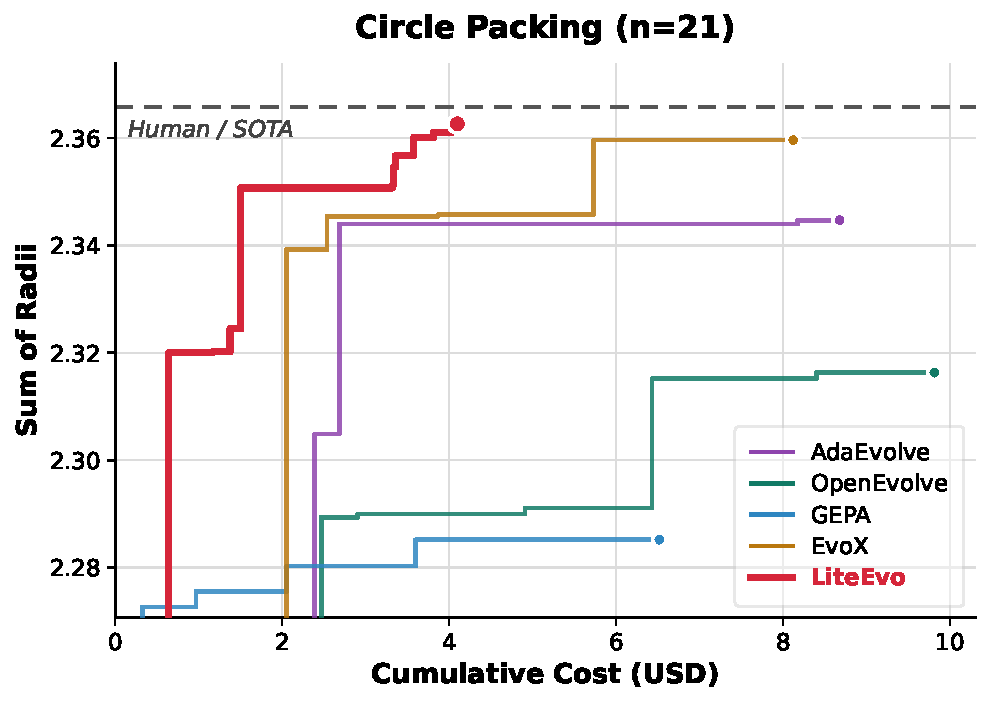
\includegraphics[width=\linewidth]{figures/frontier_circle.pdf}
\caption{\textbf{Circle packing ($n{=}21$).} Best sum-of-radii vs.\ cumulative
cost. \liteevo{} (red) reaches near-SOTA first and stops at \$4.1, while
baselines spend $1.6$--$2.4\times$ more for equal-or-lower quality.}
\label{fig:frontier-circle}
\end{figure}

\begin{figure}[t]
\centering
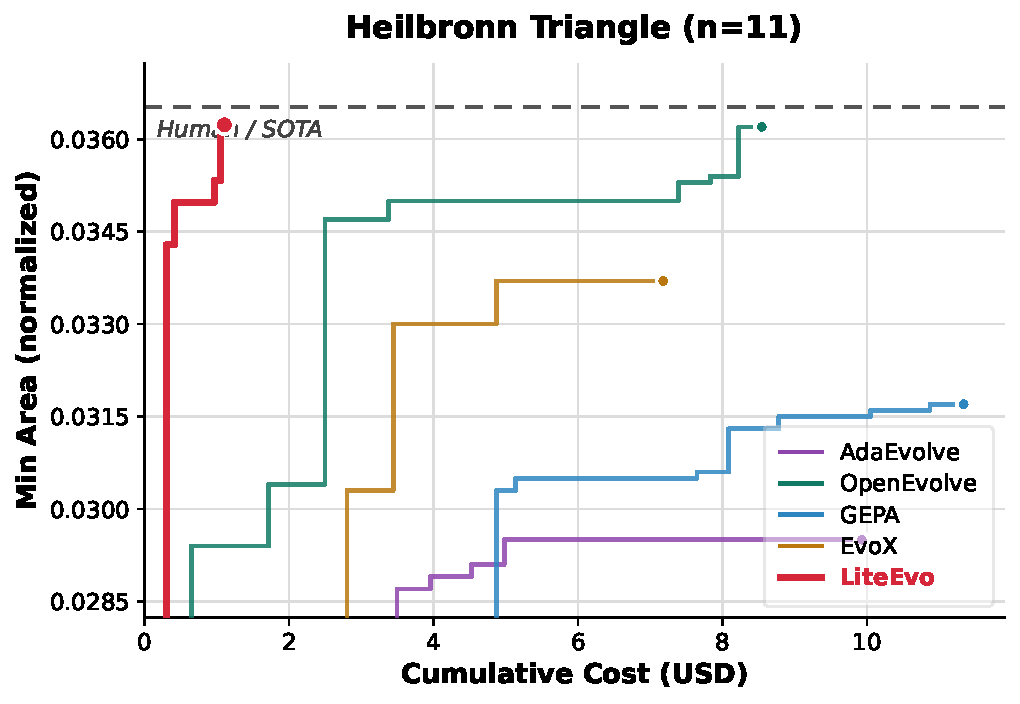
\includegraphics[width=\linewidth]{figures/frontier_heilbronn.pdf}
\caption{\textbf{Heilbronn triangle ($n{=}11$).} \liteevo{} attains $99.2\%$ of
SOTA at \$1.1 --- about $8\times$ cheaper than OpenEvolve, the only baseline that
reaches a comparable score.}
\label{fig:frontier-heilbronn}
\end{figure}

On circle packing, \liteevo{} attains $99.9\%$ of SOTA at \$4.10, versus
\$6.5--\$9.8 for the baselines; the closest baseline in quality (EvoX, $99.7\%$)
costs nearly double. On Heilbronn the gap is starker: \liteevo{} reaches
$99.2\%$ of SOTA at \$1.11, while the only baseline to match its quality
(OpenEvolve, $99.0\%$) spends \$8.54 --- a $7.7\times$ cost difference --- and the
remaining baselines plateau well below SOTA despite spending more.
Figure~\ref{fig:packings} shows the best circle-packing solutions; \liteevo{}'s
packing is visibly the tightest.

\begin{figure*}[t]
\centering
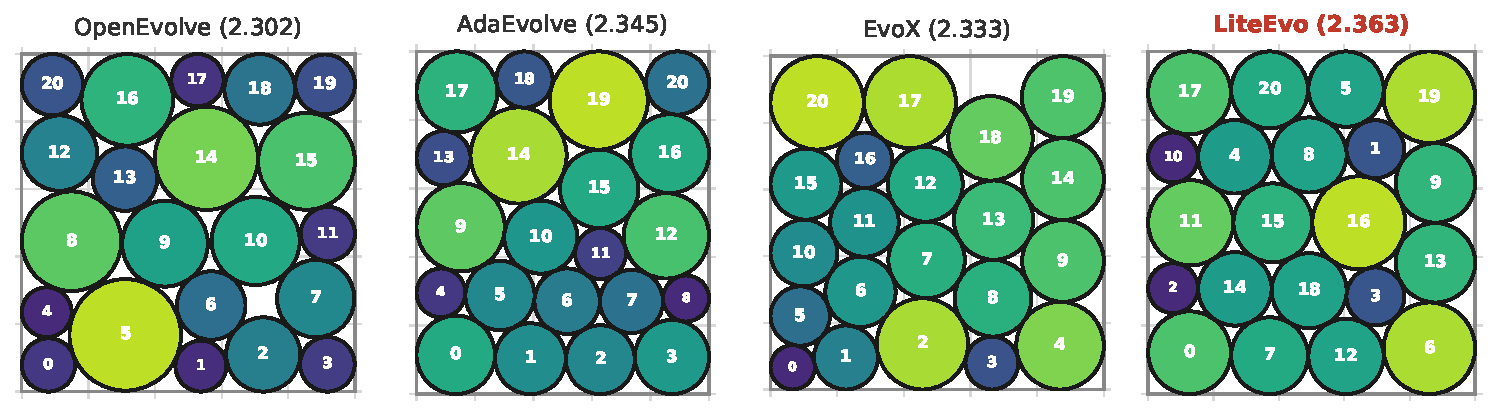
\includegraphics[width=\textwidth]{figures/best_packings.pdf}
\caption{\textbf{Best circle packings found ($n{=}21$).} Circles coloured by
radius (viridis); the title reports the sum of radii. \liteevo{} (right) packs
closest to the SOTA reference.}
\label{fig:packings}
\end{figure*}

% ===========================================================================
\section{Analysis and Ablations}
\label{sec:ablation}

\subsection{Which prompts drive progress?}
A natural worry with a small mutation model is that improvements come from one
lucky operator. Figure~\ref{fig:prompt} shows the share of \emph{new-best}
discoveries attributable to each evolutionary prompt type, averaged over six
runs (the seeding prompt is excluded). Progress is spread broadly across all
seven operators ($11$--$19\%$ each), with focused-fix mutation and structural
crossover leading. No single template dominates --- evidence that
prompt-template \emph{diversity}, not a single strong operator, is what keeps
the cheap model productive.

\begin{figure}[t]
\centering
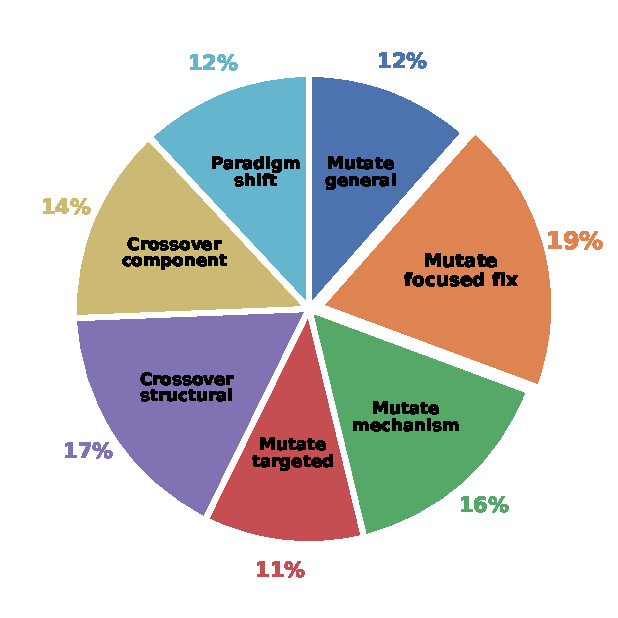
\includegraphics[width=0.86\linewidth]{figures/prompt_efficiency.pdf}
\caption{\textbf{Prompt-type efficiency.} Share of new-best discoveries per
evolutionary prompt type (mean over six runs, seeding excluded). Productivity is
spread across operators rather than concentrated in one.}
\label{fig:prompt}
\end{figure}

\subsection{Archive and cadence hyperparameters}
\liteevo{} exposes two numeric knobs that govern its cost/quality trade-off:
the paradigm-shift cadence $\tau$ (how often the frontier model is consulted)
and the number of archive cells $K$ (behavioural granularity). Larger $\tau$
spends less on the frontier model but risks under-exploring; larger $K$ gives
finer niching at the cost of slower archive turnover. We sweep both and report
their effect on final score and cost. % TODO: insert sweep table/figure once
                                       % blade_param.yml runs complete.

% ===========================================================================
\section{Conclusion}
\label{sec:conclusion}

We presented \liteevo, a cost-efficient evolutionary search for scientific
algorithm discovery with LLMs. By delegating routine variation to a small model
and reserving a frontier model for rare, plateau-breaking paradigm shifts ---
over a hybrid structure/semantics archive that sustains diversity cheaply ---
\liteevo{} matches or exceeds strong open baselines at several times lower cost,
reaching $99\%$+ of the human/SOTA reference on two mathematical-discovery
benchmarks. The broader lesson is that \emph{where} expensive model calls are
spent matters more than how many are made: allocating the frontier model by
need turns cost from a fixed tax into a tunable resource.

% ===========================================================================
\section*{Reproducibility}
All runs use fixed budgets and publicly available models. Log-extraction and
plotting scripts (producing every figure and table number here) are released
with the code. Reported baseline scores are the best programs from each run;
we note that re-executing a saved best program can yield a slightly lower score
than the run-time evaluation due to floating-point divergence across CPU
architectures, which does not affect the relative cost/quality ordering.

\end{document}
